\begin{itemize}
    \item \textcolor{blue}{Provider} Server, welche Services anbieten
    \item \textcolor{blue}{Consumer} sind Clients oder Server, die Services beziehen/benötigen
\end{itemize}

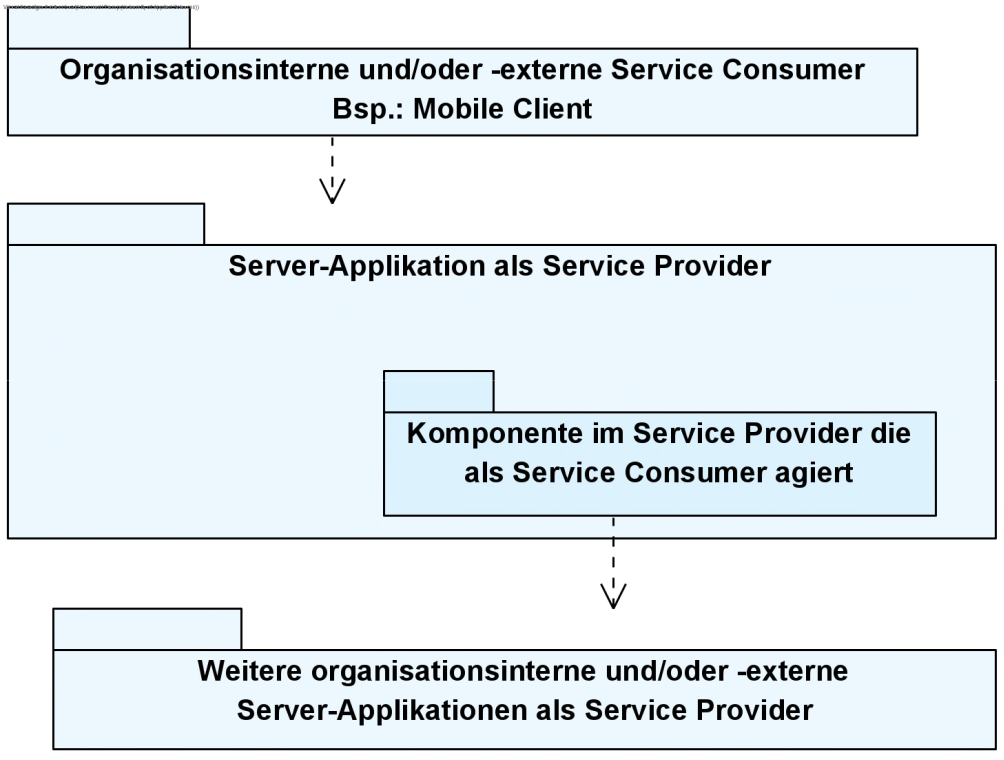
\includegraphics[width=\linewidth]{introduction2-client-server-model.png}


\subsection{SOA-enabled Mehrschichtenarchitektur (N-Tier-Architecture)}

\subsubsection{Client-/Front-End-Tier (Layer)}

Ermöglicht dem Anwender die Interaktion mit dem IT-System über eine Benutzerschnittstelle

\begin{itemize}
    \item Container: Web Browser for Web Apps
\end{itemize}

\subsubsection{Server Tiers (Layers)}

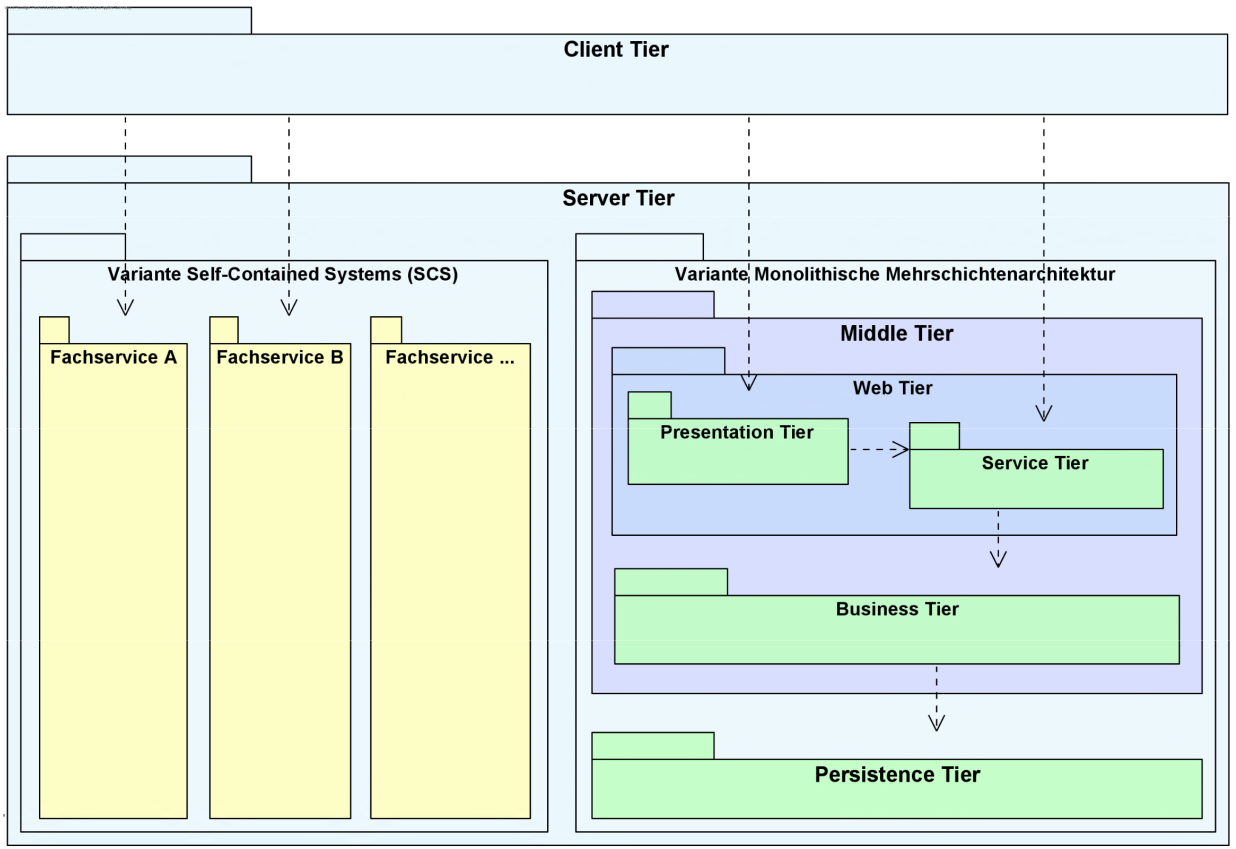
\includegraphics[width=\linewidth]{introduction2-client-server-tiers.png}

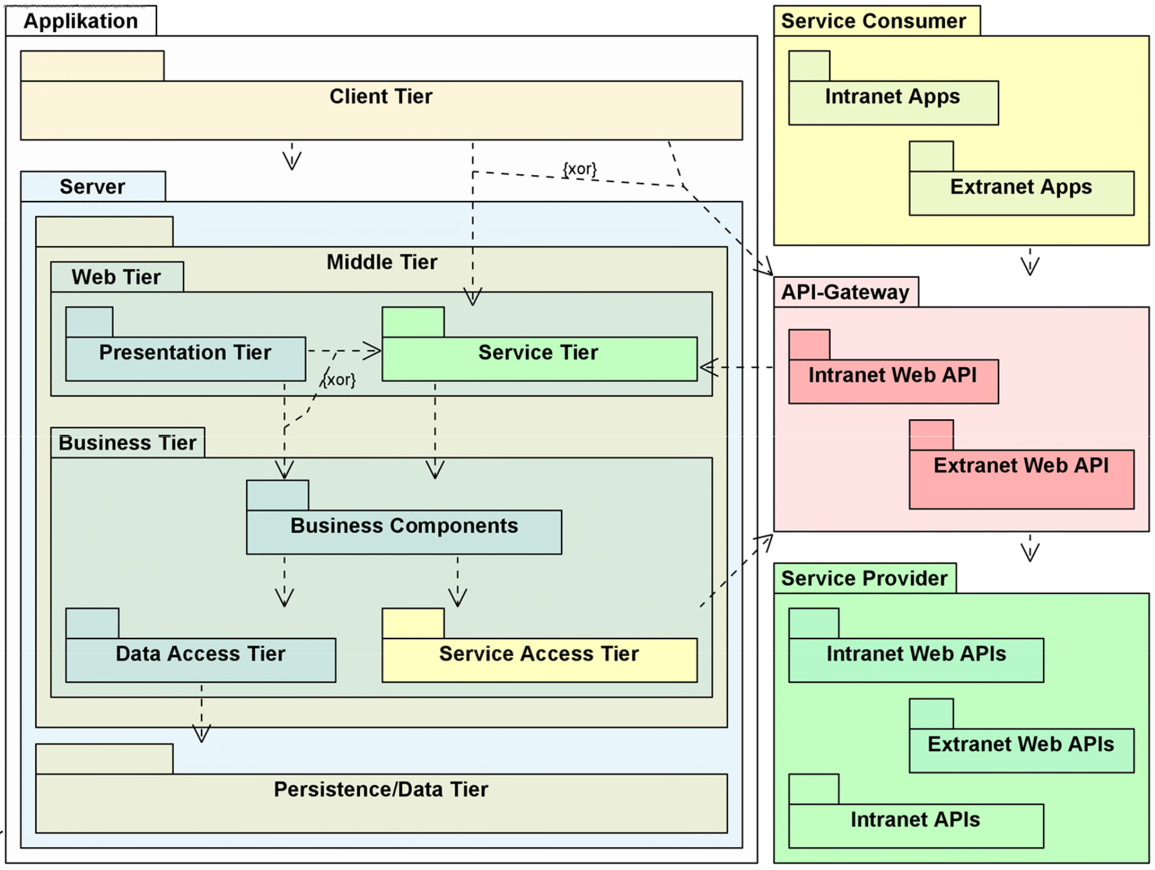
\includegraphics[width=\linewidth]{introduction2-n-tier-architecture.png} \\

\textbf{Middle-/Business-Tier (Layer)}

\begin{itemize}
    \item \textcolor{blue}{Web Tier} Präsentation, Services, bietet die Schnittstelle zum Server an
        \begin{itemize}
            \item \textcolor{blue}{Presentation Tier} Für Web Apps, welche die  View-Aufbereitung auf dem Server vornehmen. Interagiert mit dem Webbrowser.
            \item \textcolor{blue}{Service Tier} Zugriff über Web API für Service Consumer geben, meist REST oder neuerdings GraphQL, vorgelagertes API-Gateway, bildet die Service-Zugriffsebene von ausserhalb der Applikation. Damit lassen sich anderen gezielt Daten oder Funktionalität zur Verfügung stellen.
        \end{itemize}
    \item \textcolor{blue}{Business Tier} Facade für kontrollierten Zugriff, Herzstück: Business Components / Businesslogik, enthält die Geschäftslogik
        \begin{itemize}
            \item \textcolor{blue}{Data Access Tier} Access Facade, trennt sauber die in der betreffenden Fachapplikation gehaltene Persistenz, Entkoppelung der Business Komponente von DBMS-spezifischem Code (Bsp. .NEt Entity Framework)
            \item \textcolor{blue}{Service Access Tier} entkoppelt externe Service-Schnittstellen von den Business-Komponenten. Kann direkt oder über API-Gateway auf Service Provider zugreifen. Hier ist je aufgerufene externe Schnittstelle eine Proxy-Komponente zu entwickeln.
        \end{itemize}
\end{itemize}
\vspace{10pt}
\textbf{Data-/Persistence-Tier (Layer)}

speichert die Datenobjekte, hält Datenobjekte persistent, Datenbank Management(system)

\begin{itemize}
    \item \textcolor{blue}{CRUD Model} Create-Read-Update-Delete \\
    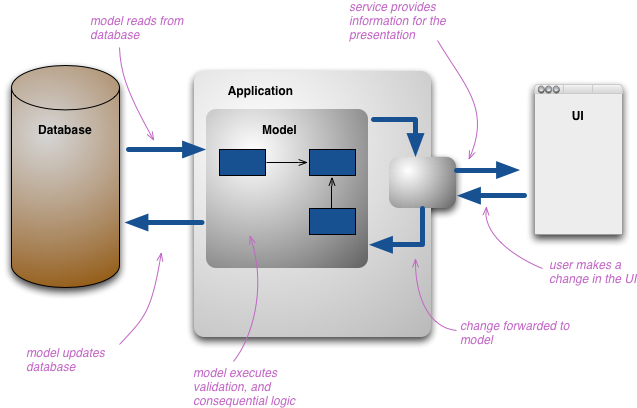
\includegraphics[width=\linewidth]{introduction2-crud}
    \item \textcolor{blue}{CQRS} Command Query Separation \\
    Das System trennt abfragenden von verändernden DB-Befehlen. Read-Befehle werden in einem Query Handler verarbeitet und in einer replizierten DB-Instanz ausgeführt, CUD-Befehle werden vom Command Handler verarbeitet und im Primary DBMS (exklusiv für verändernde Befehle) ausgeführt. \\
    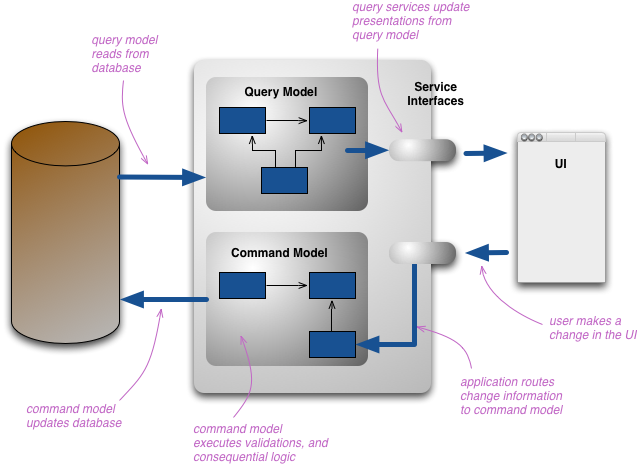
\includegraphics[width=\linewidth]{introduction2-cqrs.png}
\end{itemize}
\vspace{10pt}
\textbf{Event Sourcing (ES)}

ein Verfahren, bei dem alle Veränderungen des Zustands einer Softwareanwendung als Sequenz von Events abgebildet und aufgezeichnet werden. Er holt sich das nächste verfügbare DB-
Ereignis, um die entsprechenden DB-Befehle in der Primary DBMS ausführen zu lassen. Sobald der SQL-Befehl erfolgreich verarbeitet wurde, holt er den nächsten Befehl usw.

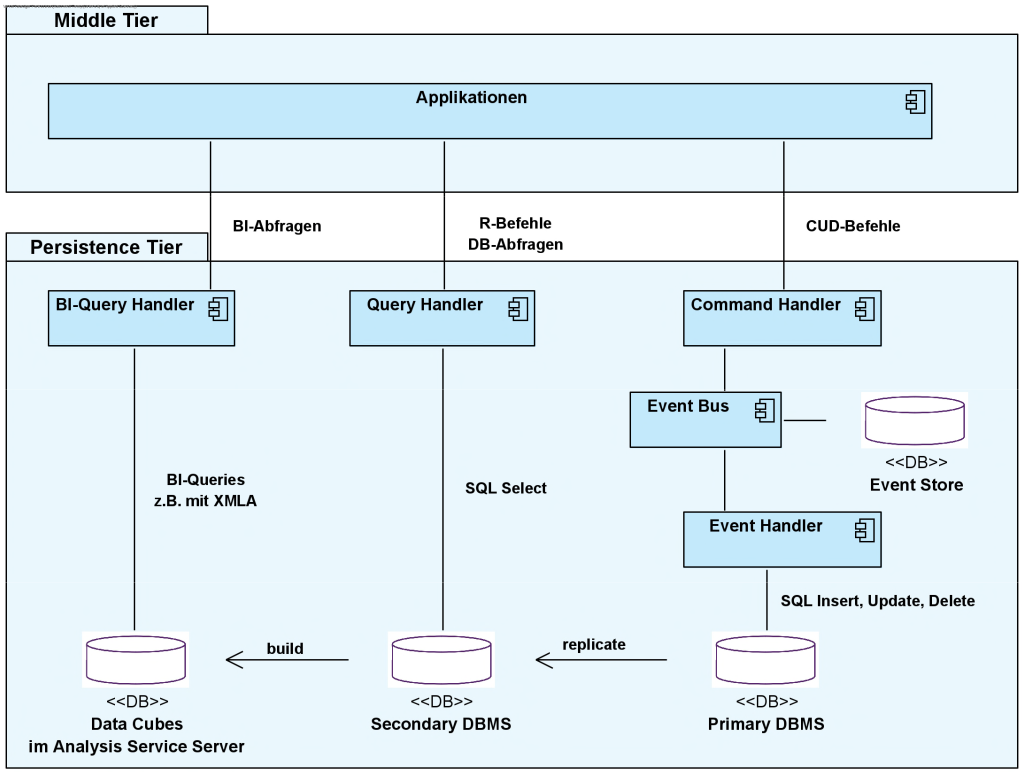
\includegraphics[width=\linewidth]{introduction2-es.png}

\subsection{Cloud}

\begin{itemize}
    \item Kosten fallen gemäss den reservierten oder effektiv genutzten Ressourcen an
    \item IT wächst oder schrumpft zeitnah mit der Unternehmung
    \item Angebotenen Dienste sind jeweils auf dem aktuellen Stand
    \item Mitarbeiter können ortsunabhängig auf die Dienste zugreifen
    \item Server in der Cloud sind sicher und hoch verfügbar
    \item Unternehmung kann sich auf ihr Kerngeschäft konzentrieren
\end{itemize}

\subsubsection{Liefermodelle (Deployment Models)}

\textbf{On Premise}

Gesamte Infrastruktur lokal installiert, über LAN miteinander und über ISP mit dem Internet verbunden. \\

\textbf{Cloud}

\begin{itemize}
    \item \textcolor{blue}{Private Cloud} Unternehmung hat alle Cloud-Ressourcen in eigener Kontrolle. Skalierung ist dabei eingeschränkt und die zugeordneten Ressourcen sind unabhängig von der Auslastung zu bezahlen.
    \item \textcolor{blue}{Community Cloud} Beispiel ist die SWITCHdrive
    \item \textcolor{blue}{Public Cloud} Ressourcen lassen sich flexible skalieren. Systeme sind öffentlich zugänglich und müssen miteinander geteilt werden. Sicher-
    heitsmechanismen schützen die jeweiligen Privatsphäre
    \item \textcolor{blue}{Hybrid Cloud} Grundlast als Private Cloud konfiguriert. Gibt es Überlast, kann das System über die Public Cloud skalieren.
\end{itemize}

\subsubsection{Serviceklassen}

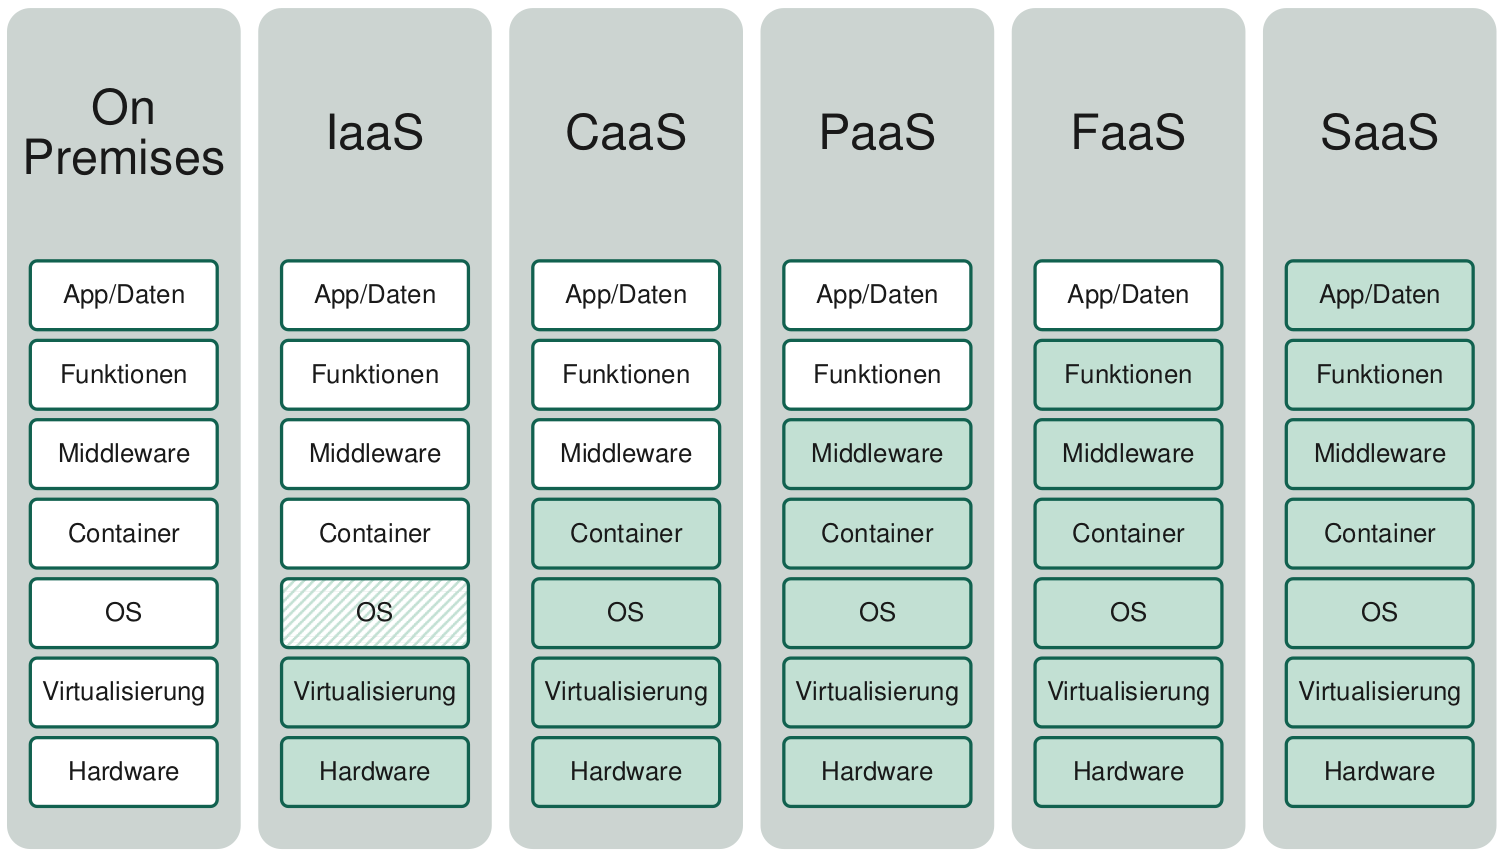
\includegraphics[width=\linewidth]{introduction2-cloud-service-classes.png}

Weiss $\rightarrow$ übernimmt der Kunde die Verantwortung
Grün $\rightarrow$ stellt der Cloud-Anbieter zur Verfügung

\begin{itemize}
    \item \textcolor{blue}{IaaS} Infrastructure as a Service, Skalierbare VM (virtuelle Maschinen), Cloud-Anbieter stellt virtuelle Maschinen mit frei konfigurierbarer Kapazität zur Verfügung
    \item \textcolor{blue}{CaaS} Container as a Service, Für die Installation von SCS, wie z.B. Microservices stellt der Cloud-Betreiber Container im Rahmen von Docker bzw. Kubernetes zur Verfügung.
    \item \textcolor{blue}{PaaS} Platform as a Service, Cloud-Anbieter stellt unterschiedliche Middleware, wie Runtime-Umgebung, Frameworks und ähnliches zur Verfügung (Bsp. Serverless Azure Web-Anwendung). Einzelne Dienste aus der Cloud
    \item \textcolor{blue}{FaaS} Function as a Service, Für serverlose Applikationen bedienen sich die Entwickler einer Fülle von Einzel-Funktionen. Bietet höchste Fle-
    xibilität und Skalierbarkeit. Das Beispielsweise AWS Lambda, Azure Functions, Google Cloud Functions
    \item \textcolor{blue}{SaaS} Software as a Service, Gesamte Applikation wie z.B. CRM (Customer Relationship Management) wird vollständig und betriebsbereit zur Verfügung gestellt.
\end{itemize}

\subsubsection{Prüfungsfragen}

\begin{itemize}
    \item Zeichnen Sie das Client-Server Modell mit einem UML Komponentendiagramm auf und zeigen Sie die Schnittstelle sowie die Interkation auf \\
    \textcolor{blue}{Antwort}
    \item Nennen Sie vier konkrete Eigenschaften von SCS \\
    \textcolor{blue}{lose Kopplung, wenige Abhängigkeiten, hohe Kohäsion, wohldefinierte Aufgabe}
    \item Welche Schichten enthalten der Web Tier? Welche Funktionen übernehmen diese und welchen Gesamtzweck hat der Web Tier? \\
    \textcolor{blue}{Prasentation Tier (innerhalb Applikation) und Service Tier (ausserhalb Applikation). Bietet Schnittstelle zum Server an}
    \item Welche Schichten muss eine Applikation aufweisen, damit sie SOA-enabled ist? \\
    \textcolor{blue}{API-Gateway, Web Service Access Tier mit Proxy-Komponente}
\end{itemize}
